\documentclass[conference]{IEEEtran}
\IEEEoverridecommandlockouts
% The preceding line is only needed to identify funding in the first footnote. If that is unneeded, please comment it out.
\usepackage{cite}
%\usepackage{natbib}
\usepackage{amsmath,amssymb,amsfonts}
\usepackage{algorithmic}
\usepackage{graphicx}
\usepackage{textcomp}
\usepackage{xcolor}

\makeatletter
\let\cite\relax
\DeclareRobustCommand{\cite}{%
	\let\new@cite@pre\@gobble
	\@ifnextchar[\new@cite{\@citex[]}}
\def\new@cite[#1]{\@ifnextchar[{\new@citea{#1}}{\@citex[#1]}}
\def\new@citea#1{\def\new@cite@pre{#1}\@citex}
\def\@cite#1#2{[{\new@cite@pre\space#1\if\relax\detokenize{#2}\relax\else, #2\fi}]}
\makeatother

\begin{document}

\title{
Discovering, recognizing, and localizing dynamic affordances to adapt to unknown agents
\thanks{This work is supported by the French National Research Agency in the framework of the "Investissements d’avenir” program (ANR-15-IDEX-02).}
}

\author{\IEEEauthorblockN{Simon L. Gay}
\IEEEauthorblockA{\textit{LCIS, Univ. Grenoble Alpes} \\
Valence, France \\
simon.gay@lcis.grenoble-inp.fr}
\and
\IEEEauthorblockN{Jean-Paul Jamont}
\IEEEauthorblockA{\textit{LCIS, Univ. Grenoble Alpes} \\
Valence, France \\
Jean-Paul.Jamont@lcis.grenoble-inp.fr}
\and
\IEEEauthorblockN{Olivier L. Georgeon}
\IEEEauthorblockA{\textit{EA1598, Lyon Catholic University} \\
\textit{LIRIS, Claude Bernard University} \\
Lyon, France \\
ogeorgeon@univ-catholyon.fr}
}

\maketitle

\begin{abstract}
We present an architecture for self-motivated and environmentally-agnostic agents to integrate non-predictible elements in their emerging model of their environment. This approach aims designing agents that construct their own model of their environment through experience, rather than exploiting pre-coded knowledge. Over time, the agent learns the relation between its perception of objects and the interactions that they afford, in the form of data structures, called signatures of interaction. These signatures are used to recognize and localize objects (or affordances) in surrounding environment, that are stored and tracked in a spatial memory, and used to generate behaviors satisfying agent's motivational principles. A long term objective of this approach is to study the interaction between multiple agents and the emergence of collaborative or competitive behaviors. Emergence of such behaviors requires the possibility to integrate other agents in the environment model and predict possible actions of these agents. In this paper, we propose a novel architecture of signature of interaction that can define, recognize and localize non-predictable affordances.
\end{abstract}

\begin{IEEEkeywords}
developmental learning, interactionism, affordance, autonomous mental development, spatial awareness.
\end{IEEEkeywords}

\section{Introduction}\label{intro}

We address the problem of how an artificial agent that learns an emergent model of its environment through interaction can acquire knowledge about mobile entities that move freely in the environment (e.g., other agents).

This study is situated within the framework of artificial constructivist learning \cite[e.g.,][]{wang_new_2012} and enactive learning \cite[e.g.,][]{froese2009enactiveAI}.
In this framework, the learning occurs through the enaction of control loops that implement Piagetian \textit{sensorimotor schemes} \cite{piaget2013construction}, which we call \textit{interactions}.
This framework also relates to the notion of \textit{intrinsic motivation} of artificial agents for \textit{developmental learning} \cite[e.g.,][]{oudeyer:motivation}.

More precisely, we investigate a modeling hypothesis called \textit{Radical Interactionism} (RI) \cite{georgeon:radical} and \textit{artificial interactionism} \cite{GuillerminGeorgeon2022}.  
We implement a kind of self motivation called \textit{interactional motivation} \cite{georgeon_interactional_2012}.
The agent starts with a predefined set of uninterpreted \textit{interactions} associated with predefined numerical \textit{valences}, and seeks to enact interactions of positive valence and to avoid interactions of negative valence.
Overall, the learning is \textit{unsupervised}. 
There are no human-defined labels attached with perceptions, actions, or categories of entities, not even spatial localization of percepts.
% The agent has initially no \textit{a priori} knowledge about its perception nor on its environment.

Through the learing of interaction with other mobile entities,
we pursue the long-term goal of allowing the emergence of social behaviors within groups of artificial agents \cite[e.g.,][]{nsfkatz10}, for example collective hunting. Generating such behaviors requires overcoming two main problems:

1) learning to define, recognize and localize other agents that make self-motivated movements in the environment,

2) inferring the intentions of other agents based on their own environmental contexts.

This paper focuses on the resolution of the first problem. 
It is subdivided as follows: Section \ref{RI} summarizes and formalizes the Radical Interactionism model, Section \ref{signatures} presents a model for defining and recognizing probabilistic affordances, and Section \ref{localize} presents a mechanism to recognize and localize distant probabilistic affordances in space. Finally, Section \ref{conclusion} encompasses some conclusive remarks and future development of the intersubjectivity problem.




\section{The Radical Interactionist (RI) hypothesis}\label{RI}

In contrast with most machine learning approaches, an RI agent cannot directly access the state of its environment: its input data is outcome of control loops rather than percepts of the environment's state.
The agent learns and exploits regularities in sequences of control loops offered by its coupling with its environment.
The learning mechanism differs from reinforcement learning (e.g., as it is typically implemented in a Partially Observable Markov Decision Process) by the fact that RI agents have no reward defined as a function of the system's state.
Our goal is not to design agents that reach predefined goals or maximize a reward value, but to study the open-ended learning of emergent models of the environment, and to generate social behaviors.

Let $I$ be the set of predefined primitive interactions (control loops).
% and $\nu_i \in \mathbb{R}$ the predefined valence of primitive interaction $i \in I$.
At the beginning of step $t$, the agent selects an \textit{intended interaction} $i_t \in I$.
An example consists in moving forward for a predefined duration.
At the end of step $t$, the agent receives the \textit{enacted interaction} $e_t \in I$ that was actually enacted. 
If $i_t = e_t$ then the enaction is a success. 
The agent \textit{did} move forward.
Otherwise, the enaction of $i_t$ is a failure.
For example, the agent actually enacted another interaction consisting in bumping into an obstacle, which may have a negative valence.
An RI agent learns to anticipate the results of its interactions, and tries to enact interactions of high valence.

To help the agent discover that its environment has a spatial structure (2D in our experiments), we designed the Parallel-RI (PRI) model \cite{gay:space} which allows the simultaneous enaction of multiple interactions.
The PRI considers additional stimuli that cannot be separated from the movement that produced them. The optical flow is an example of such stimuli, that must be associated to a movement to characterize a position in space. Thus, the PRI model considers \textit{primary interactions} as control loops (action,result), and \textit{secondary interactions} as a couple (interaction, stimulus).
At the end of step $t$, the agent receives, not one, but a set of $k$ enacted interactions $E_t=\{e_1,..., e_k\} \subset I$, containing a primary interaction and a set of secondary interactions associated with this primary interaction.

Previous PRI experiments showed that the agent was able to define, recognize and localize affordances (possibilities of enacting an interaction \cite{gibson:affordances}), and to store and keep track of them in an emergent structure, called Space Memory \cite{gay:space}. This memory generates an implicit context of affordances that the agent can exploit to generate behaviors in accordance with its interactional motivation.
A subsequent model also showed the possibility to identify objects that moved in a straight line, by considering sequences of consecutive interactions \cite{gay:dynamic}. 
These models, however, could not integrate entities moving irregularly (other agents).
The present study addresses this limitation.



\section{Integrating Mobile Affordances}\label{signatures}

This section explains the \textit{signature mechanism} \cite{gay:space} by which the agent estimates the possibility of enacting interactions in a given context.
This mechanism is based on the assumption that the enaction result of an interaction $i$ depends on a limited context of elements in the environment, defining the \textit{affordance} of $i$. 
As a PRI agent can only perceive its environment through enacted interactions, we define the signature $S_i$ of an interaction $i$ as an emerging structure characterizing one or several sets of interactions (i.e. $\{j_k\} \subset E_{t}$) whose enaction  can characterize the presence of an element affording $i$ for next step $t+1$.

Defining objects by learning the affordances they provide is abundant in literature, e.g., 
\cite{paola:affordance, baleia:affordance, ugur:traversability}.
Most of these approaches define affordances from perception, which limits the detection to next action, or requires prior knowledge on environment and space \cite[e.g.,][]{manoury:affordance} to detect distant affordances. 
Signatures cope with this limitation by using interactions instead of perception, allowing to exploit spatial properties implicitly encoded in interactions to detect distant affordances.


Formally, a \textit{signature of interaction} is a function $S_i : \mathcal{P}(I) \rightarrow [-1;1]$, where $\mathcal{P}(I)$ is the partition of $I$, i.e., the set of all possible contexts.
$S_i(E_{t}) \in [-1, 1]$ gives the prediction of successfully enacting interaction $i$ at step $t+1$: 1 for certainty of success, -1 for certainty of failure.
%²To improve estimations, 
The agent adjusts the parameters of $S_i$ each time $i$ succeeds or fails.

Signatures must be \textit{reversible} by defining a pseudo-reverse function $\hat{S}_i : \{-1;1\} \rightarrow \mathcal{P}(\mathcal{P}(I))$ such that  $\hat{S}_i(1)$ gives the set of minimal contexts $C_l^i$ in which $i$ is possible, i.e. contexts that \textit{afford} $i$, and $\hat{S}_i(-1)$ gives the set of minimal contexts in which the enaction of $i$ is impossible.


However, when interacting with mobile entities, the presence of an affordance at the end of step $t$ does not guaranty that the interaction can be enacted during step $t+1$ because the entity may move in the meantime. 
We thus must separate the estimation of the presence of an affordance from the prediction of success of enacting the interaction.




\subsection{Separating affordances from prediction of success}\label{separate}

From an observer's perspective, three types of situations can happen when the agent tries interacting with a mobile entity:

\begin{enumerate}
\item The affordance is present at the right place, and the agent enacts the interaction successfully (e.g., a prey is in front of the agent, and the agent catches the prey).
\item The affordance is present, but the interaction fails (e.g., a prey is in front of the agent, but the prey moves and the agent fails to catch it).
\item The affordance is absent, leading to a failure of the interaction (e.g., there is not pray in front of the agent, but the agent tries to catch one and fails).
\end{enumerate}

From the agent's perspective, situations 2 and~3 cannot be distinguished, as they have the same result.
Situations 2 distorts the learning of signatures, as situations 1 and 2 can occur in the same context $E$, causing the prediction $S_i(E)$ to remain negative even though the affordance is present.


However, our preliminary tests showed that, despite remaining negative, signature predictions are slightly higher in case of situations 1-2 than in situations 3. Indeed, situations 1 allow contexts of interactions designating the affordance to emerge, while remaining insufficient to predict with a positive value.

We thus use the average prediction in case of failure $\overline{S_i^f}$ as a threshold to distinguish between situations 2 and 3.
When the interaction fails in an assumed situation 2 (i.e., $S_i(E_t)>\overline{S_i^f}$), the signature is not reinforced, which limits the influence of situations 2 in signature construction. 


Symmetrically, some interactions may fail due to the presence an entity in a specific location (e.g., trying to move forward will succeeds unless an obstacle appears).
As success of such interactions are expected to be more frequent than failures, the average of predictions will converge to a positive value.
In this case, the average of positive predictions $\overline{S_i^s}$ is used as a threshold to prevent the signature reinforcement in case of success in an assumed situation 2 (i.e. $S_i(E_t)<\overline{S_i^s}$).


It is then possible to define the ratio of success when the prediction $S_i(E_t)>\overline{S_i^f}$ (or failure when $S_i(E_t)<\overline{S_i^s}$), implying that the agent is in a situation of type 1 or 2. A ratio $p_{C_l^i}^i$ is thus defined for each context $C_l^i \in \hat{S}_i(1)$ measuring the probability that the interaction will succeed in the presence of an affordance containing a mobile entity.



\subsection{Implementation of Signatures}\label{contexts}


We extend Gay \textit{et al}'s signature architecture \cite{gay:space} using multiple neurons as illustrated in Fig. \ref{fig:neuron}. 
Each signature $S_i$ consists of $m$ neurons $N_i^1$ to $N_i^m$~; the neuron with the strongest output defines the prediction of $S_i$. 
In case of success, the neuron with the strongest output is reinforced, while a failure reinforces all neurons. 
This competition leads to a specialization of each neuron for a specific context, while they are desensitized from other contexts. Thus, with a sufficient number of neurons, a signature can identify contexts affording its interaction independently.

Formally, a neuron $N_i^n$ is defined as a set of weights $\{w_k^n\}$, with $Card(\{w_k^n\})=Card(I)$, and an output defined as:
\begin{equation}
N_i^n(E_t)~=~f(\sum_{k} E_t[k] \times w_k^n)~,~ f(x) = { {1}\over{1+e^{-x} }}
\end{equation}
where $E_t[k]=1$ when $i_k \in E_t$ and $E_t[k]=0$ otherwise.

Then, the response of the group is defined as the maximum output, and remapped to a range in $[-1;1]$:
\begin{equation}
N_i(E_t)~=~max_n (N_i^n(E_t) ) \: \times \: 2 ~+~ 1
\end{equation}
In order to consider interactions that are afforded by the absence of an entity instead of its presence, we added an output weight $W_i$ defining the output of the signature:
\begin{equation}
S_i(E_t)~=~N_i(E_t) \times W_i
\end{equation}
The weight $W_i$ is restrained in the interval $[-1,1]$, allowing to inverse the result of the prediction, which makes neurons able to integrate contexts preventing the enaction of $i$.

The learning process uses a classical gradient descent\footnote{The enaction result of $i_t$ is defined as $r_t=1$ in case of success ($i_t \in E_t$) and $r_t=-1$ in case of failure ($i_t \not\in E_t$).
The weight $W_i$ is updated as follows:
$W_i ~\Leftarrow~ W_i+ \Delta_i . (\alpha * N_i - \alpha /2)$, ~with $\Delta_i = r_t - S_i(E_{t-1})$
and $\alpha$ the learning rate.
In case of success, only the neuron with the highest output is reinforced.
In case of failure, all neurons are reinforced:
$w_k^n ~\Leftarrow~ w_k^n+ \alpha . \Delta_i^n . N_i^n$,
with $\Delta_i^n=(r_t.W_i + 1)/2 - N_i^n$.}
and prediction values obtained with $E_{t-1}$.

A consequence of this implementation is that high weights of neurons characterize contexts affording $i$.
Weights of neurons can be grouped by primary interaction, each group containing a weight related to a primary interaction and weights related to its associated secondary interaction. 
Thus, a signature $S_i$ can be subdivided into minimal contexts $C_{j,n}^i$, associated with a primary interaction $j$ and a neuron $n$. 
It is then possible to define the ratio of success $p_{j,n}^i$ of each context $C_{j,n}^i$ by updating it when $j \in E_{t-1}$ and neuron $n$ has the highest activity, and $S_i(E_{t-1})<\overline{S_i^s}$.

\begin{figure}[htbp]
\centerline{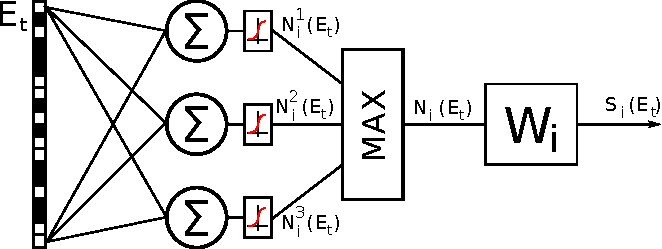
\includegraphics[scale=0.55]{img/signature_model2.pdf}}
\caption{Signature architecture based on multiple neurons. As the signature output relies on the neuron with the greatest output, neurons are in competitions, leading to a specialization of each neuron for a specific context. The last function remaps the output to range $[-1;1]$ and uses a global weight $W_i$, that can inverse the signature result, allowing the representation of contexts preventing the enaction of an interaction.}
\label{fig:neuron}
\end{figure}

\subsection{Test Environment}\label{implementation}

This signature mechanism was tested on an artificial agent moving in the 2-dimensional discrete environment shown in Fig.~\ref{fig:environment}.
The sensorimotor possibilities of the agent define the following five primary interactions:

 \begin{tabular}{ l l }
   - 
\includegraphics[width=0.015\textwidth]{img/mf0.pdf} \textit{move forward} by one step, \\
   - 
\includegraphics[width=0.015\textwidth]{img/mf1.pdf} \textit{bump} in a solid element, &
   - 
\includegraphics[width=0.02\textwidth]{img/lt0.pdf} \textit{turn left} by $90^\circ$\\
   - 
\includegraphics[width=0.015\textwidth]{img/mf2.pdf} \textit{eat} something edible, &
   - 
\includegraphics[width=0.02\textwidth]{img/rt0.pdf} \textit{turn right} by $90^\circ$\\
 \end{tabular}

Interactions \textit{move forward}, \textit{bump} and \textit{eat} are considered as mutually alternative: intending one of these interactions may lead to the enaction of one of the two others instead.

We add a set of secondary interactions provided by the agent’s visual system, that can detect colors and measure distances, with a field of view of 180°.
Secondary interactions consist in \textit{seeing} the displacement of a red, green or blue entity at a certain (but unknown) position in egocentric space, while enacting a primary interaction.
Interaction \textit{bump} does not generate visual interactions (no movement).
We discretize the visual field as a grid of 15 × 8 positions in front of the agents that matches the environment's grid.
We thus define 4 × 3 × 15 × 8 = 1440 secondary interactions.
Signatures are implemented using sets of $m=6$ neurons.
The signature learning process is driven by a learning mechanism that foster interactions with low certainty of success or failure (low $|S_i(E_t)|$).

The environment contains three types of objects offering spatial regularities that the agent can discover by interacting with them, and characterized by a color that makes them recognizable through its sensorimotor system: 1) wall (green), affording bump, 2) algae (red), that are walkthroughable (and thus useless in the agent's perspective), and 3) fish (blue), affording eat.
The fish move randomly: at each simulation step, they can stay immobile, or move left, right, up, or down, with a probability of 20\% each.
If the fish cannot move in the selected direction because of an obstacle (wall, alga or other fish), it remains immobile, making the immobile situation slightly more probable than other directions. This random movement simulates agents with unknown behavior.

\begin{figure}[htbp]
\centerline{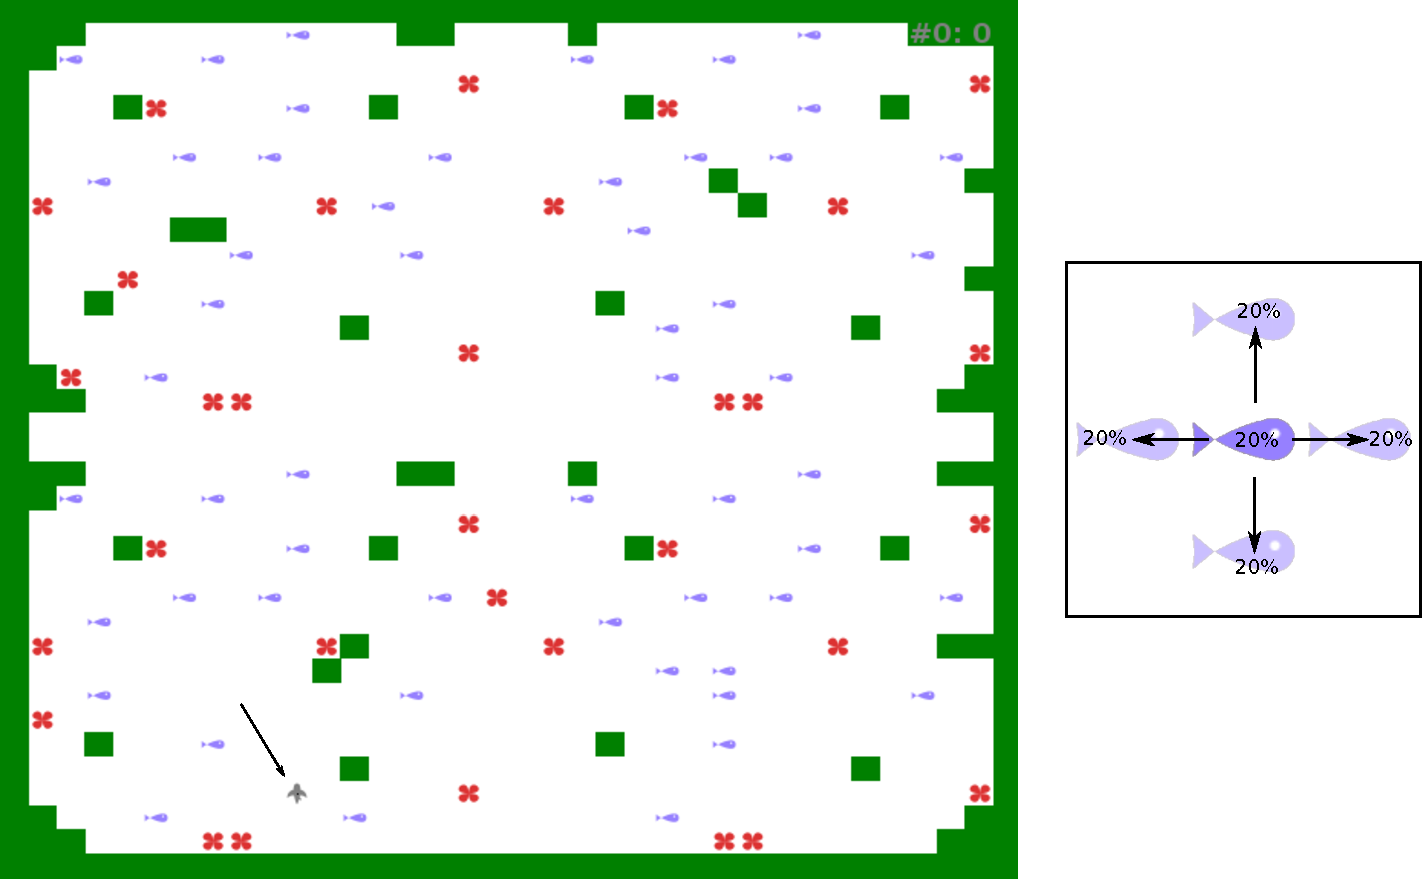
\includegraphics[scale=0.28]{img/environment.pdf}}
\caption{Test environment. The agent is represented as a grey shark (bottom left), wall as green blocks, algae as red leafs and mobile preys as blue fishes. At each simulation step, the fish has 20\% of remaining at current position or to move up, down, left, or right.
}
\label{fig:environment}
\end{figure}




We then let the agent behave in its environment, driven by the signature learning mechanism. 
Signature of bump (Fig.~\ref{fig:bump}) emerges and stabilizes within 5000 simulation steps. 
The signature is similar to signatures obtained in previous environments \cite{gay:space}\cite{gay:dynamic}.
It associates the success of \textit{bump} with the presence of \textit{seeing a green element moving right in front of the agent}, and of a previously enacted \textit{bump}. 
The signature thus gathered every interaction allowing to detect the presence of a wall in front of the agent, even through they come from different sensory modalities.

\begin{figure}[ht]
\centerline{\includegraphics[scale=0.35]{img/Signatures1_5.pdf}}
\caption{Signatures of interaction \textit{bump} after 100 000 steps. 
It is characterized by the weights of 6 formal neurons, each neuron being represented by a column. 
As the signature identified a unique context, we only represent weights of one neuron. 
As en external observer, knowing that the environment is 2D, we organize weights of a neuron to make signatures more readable: first, weights associated with primary interactions are represented with five squares below (green for a positive weight, red for a negative weight). 
Weights associated with secondary interactions are grouped according to their primary interactions, forming the four groups (from top to bottom: forward, eat, turn left, turn right ; bump does not produce visual interactions). 
Each group is organized to place visual interactions with their associated position in space, relative to the agent (orange triangle). 
Colors associated with visual interactions are overlapped to generate signatures under the form of a RGB image. 
Signature of bump identified a context that consist of seeing a green element in front of the agent, which corresponds to the presence of a wall in front of the agent. 
Bump is also related to the success of previous bumps, since the agent can bump repeatedly.
}
\label{fig:bump}
\end{figure}



Signatures of secondary interactions related to static elements (\textit{seeing red} and \textit{seeing green}) progressively stabilize, depending on their frequency of occurrence. 
After 50 000 simulation steps, most of these signatures stabilized. 
These signatures are also similar to signatures obtained with static entities \cite{gay:space}\cite{gay:dynamic}. 
They designate elements of the same color but on a different position in space. 
From an external point of view, the spatial offset between the visual interaction and the entity designated by its signature matches the movement performed by the enaction of its associated primary interaction. 
This property is used for distant affordance detection \cite{gay:space} (details in Section \ref{localize}).


Signatures of interactions related to mobile elements require more steps, as they relate to a larger variety of contexts to identify: at least 45 000 steps are required to identify contexts affording \textit{move forward} and \textit{eat}.
Signature of interaction \textit{eat} (Fig.~\ref{fig:eat}) characterizes five contexts corresponding to the five positions of fish that can lead to a success of eat. 
Note that the position under the agent does not appear in contexts of interactions associated to move forward, as this situation is not possible. 
The signature of \textit{move forward} (Fig.~\ref{fig:forward}) has a negative weight $W$. 
The signature thus shows the affordance that prevents this interaction. 
The signature designates five contexts associated with the presence of a fish, and one context associated with the presence of a wall in front of the agent.

Signatures of secondary interactions consisting in seeing blue (Fig.~\ref{fig:sigblue}) elements designate five contexts, corresponding to the five positions leading to a success of these interactions, with an offset (from an external point of view) corresponding to the movement of the associated primary interaction.

\begin{figure}[ht]
\centerline{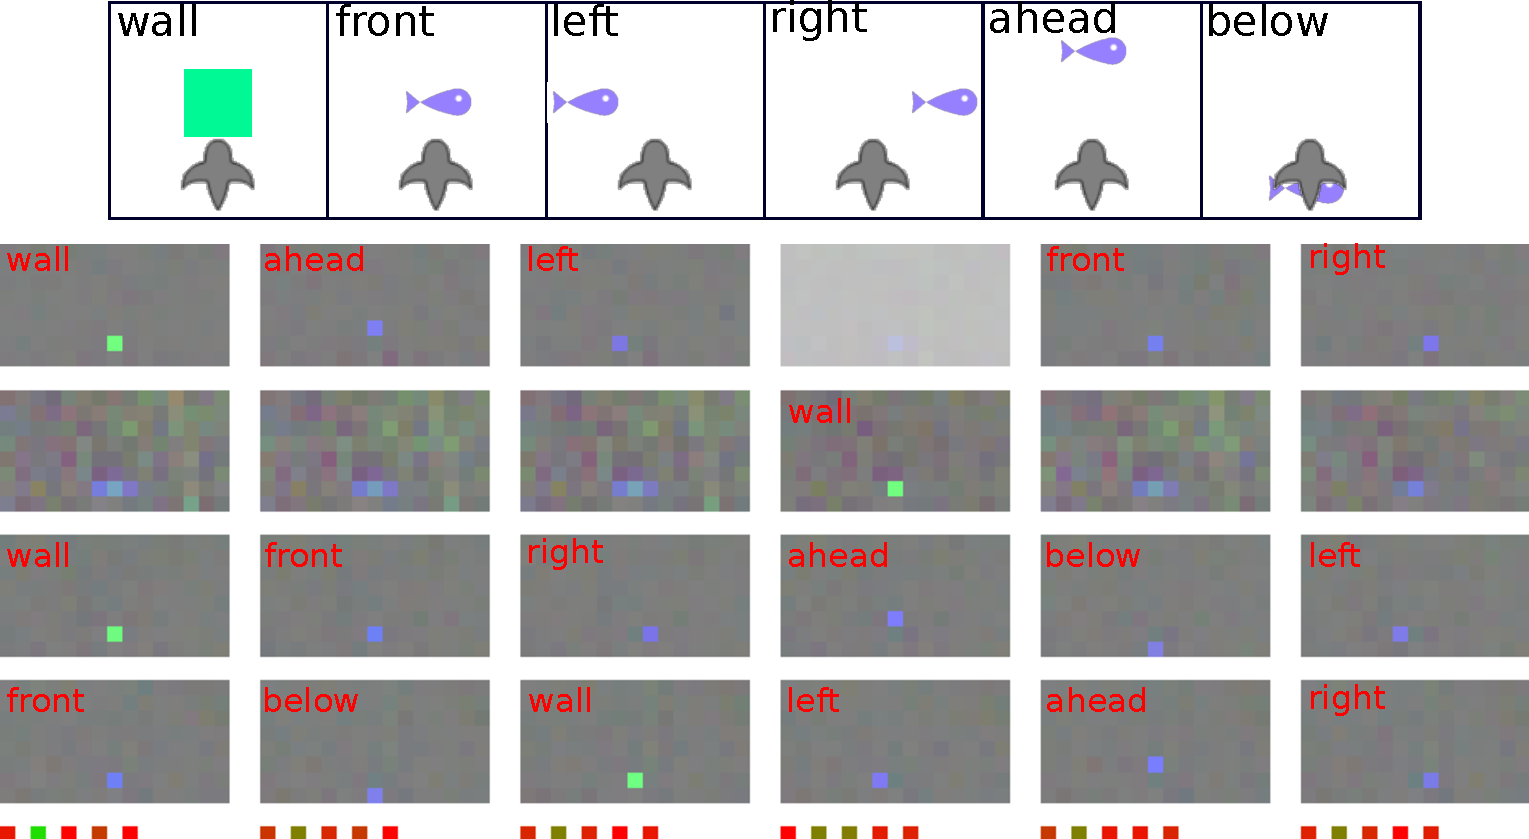
\includegraphics[scale=0.32]{img/sig_forward.pdf}}
\caption{Signature of \textit{move forward}, recorded after 100 000 simulation steps. Each column represents a neuron of the signature. The weight W is negative: the signature thus represents contexts \textit{preventing} moving forward. The signature identifies six contexts, represented (from an external point of view) above. As a fish cannot be below the agent after forward or eat, only 5 contexts are related to forward primary interaction (greyed context has low weights and is thus unused by the signature). As eat interaction is rarely enacted, contexts related to this primary interaction (second line) are still constructing.
}
\label{fig:forward}
\end{figure}



\begin{figure}[t]
\centerline{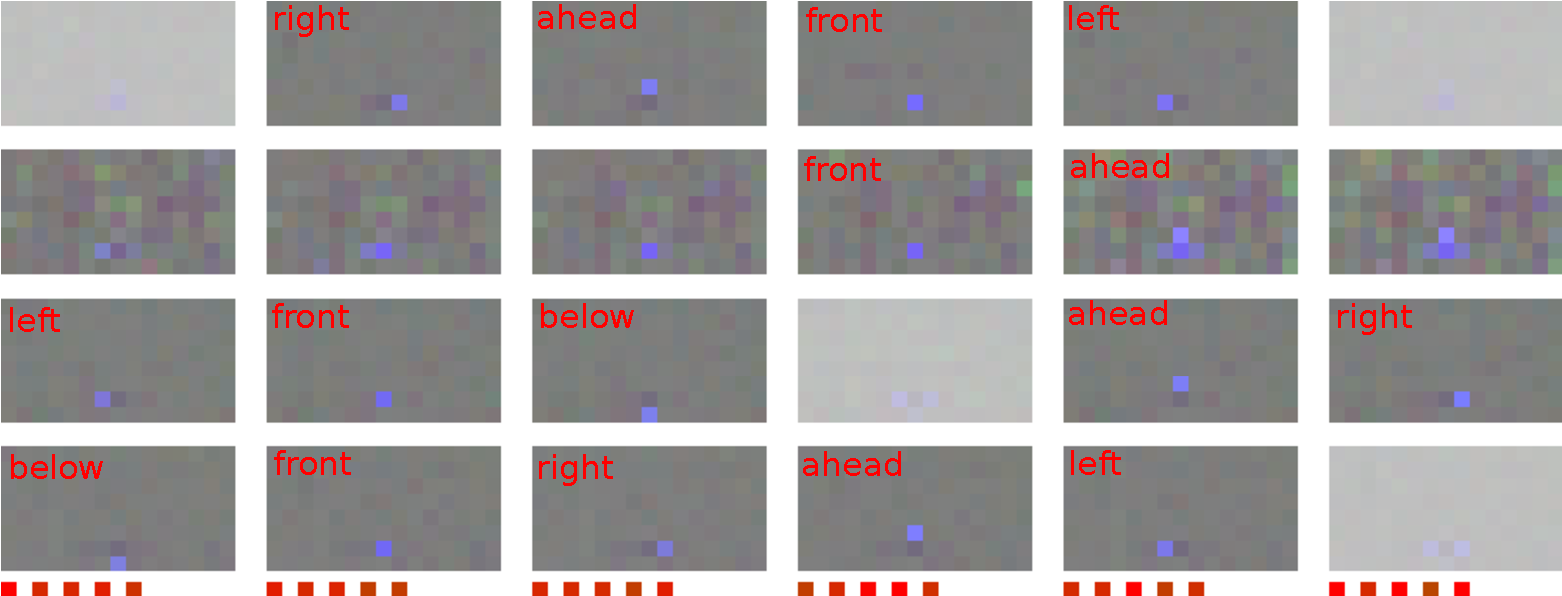
\includegraphics[scale=0.32]{img/sig_eat.pdf}}
\caption{Signature of eat. The weight W is positive.
The signature identifies 5 configurations of fish (front, ahead, left, right, below), 4 in the case of a move forward (as below context cannot be observed). In contexts with fish around front position, we can observe the absence of a green or red element (dark blob) in front of the agent, as this would prevent the prey from moving to this position.}
\label{fig:eat}
\end{figure}

\begin{figure}[t]
\centerline{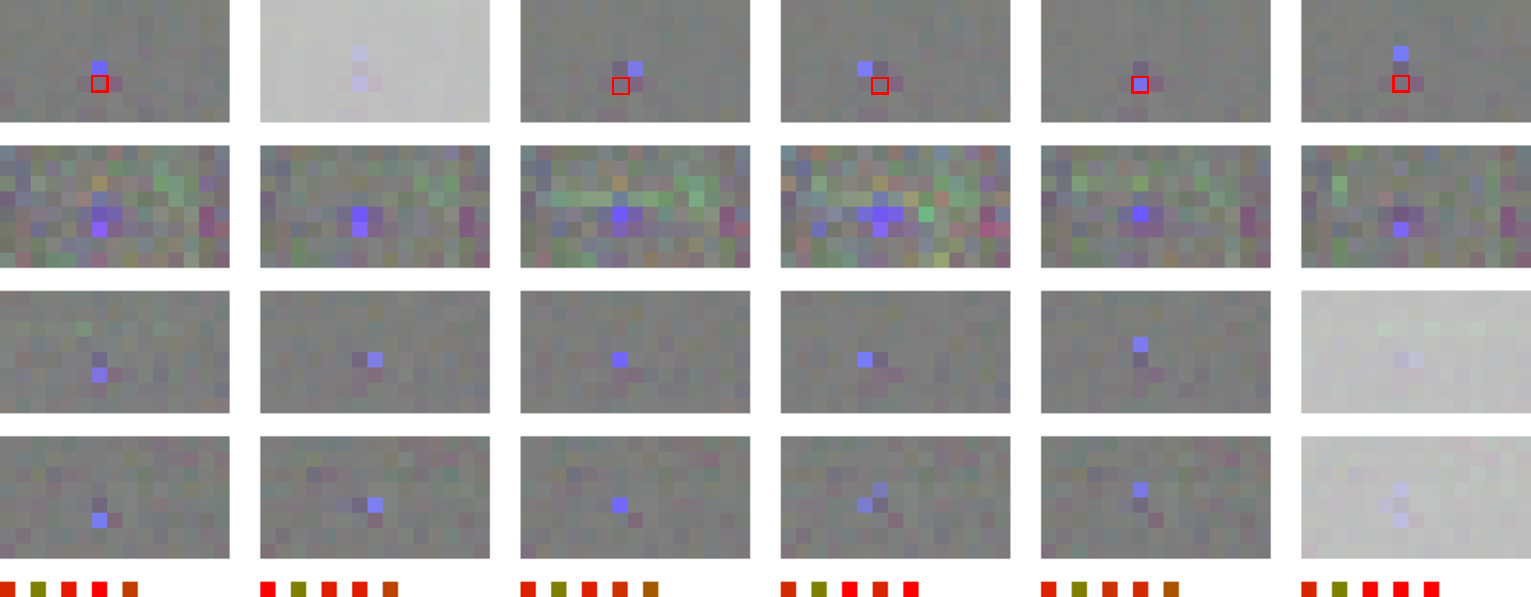
\includegraphics[scale=0.32]{img/sig_blue.pdf}}
\caption{Signature of secondary interaction seeing a blue element at the position identified with a red square, while moving forward. The weight W is positive. The signature identifies 5 configurations of fish. The signature also indicates the absence of an element that would prevent the fish from moving on the right place, but also elements that could hide the fish (dark blobs).}
\label{fig:sigblue}
\end{figure}


We also analyze the ratio of successful enaction after a prediction of success. 
The ratios obtained in contexts implying static objects (such as walls) are close to 1 indicating that the presence of this type of affordance implies the success of the interaction. 
Ratios obtained with mobile fish are close to 20\%, which correspond to the probability that the fish moves in the right direction when the agent tries to eat it. 
The contexts with a fish in front of the agent is however slightly greater. 
This can be explained by the fact a prey cannot move to a different position when blocked by a wall or an alga, increasing the probability of eating the fish when in front of the agent. 
These ratios, summarized in table \ref{tab1}, show that signatures can integrate and encode stochastic properties of the environment.


\begin{table}[htbp]
\caption{Average ratios of successful prediction in contexts: wall, fish in front, and fish in other positions (surrounding)}
\begin{center}
\begin{tabular}{|c|c|c|c|}
\hline
\textbf{interaction} & \textbf{\textit{wall}}& \textbf{\textit{front}} & \textbf{\textit{surround.}}\\
\hline
forward & 0.96 & 0.25 & 0.19 \\
\hline
bump    & 0.97 & /    &  / \\
\hline
eat & / & 0.24 & 0.19 \\
\hline
seeing blue (Fig. \ref{fig:sigblue}) & / & 0.24 & 0.18 \\
\hline
\end{tabular}
\label{tab1}
\end{center}
\end{table}



\section{Localizing Distant Affordances}\label{localize}


The detection of distant affordances relies on a property of signatures: a signature of an interaction designates an affordance as sets of interactions ~$\{j_k\} \in \hat{S}_i(1)$ allowing to detect the presence of this affordance.
However, each interaction $j_k$ can have its own signature. 
It is thus possible to define, from these signatures $S_{j_k}$, a set of contexts, called \textit{predecessor} $\hat{S}_i^{[j]}$, that, after enacting $j$, afford $i$. 
The \textit{backmove} principle consists in defining the initial predecessor $\hat{S}_i^{\sigma_0}=\hat{S}_i(1)$, with $\sigma_0=\langle\rangle$ (empty sequence). 
Then, recursively project the predecessor $\hat{S}_i^{\sigma_a}$ with:
$\hat{S}_i^{\sigma_{a+1}}\!=\!\bigcup_{\forall C_l^i \in \hat{S}_i^{\sigma_a} / j \in C_l^i} \{E \in \mathcal{P}(I) / \forall j_k \in C_l^i, S_{j_k}(E)\!>\!0\}$,
with $\sigma_{a+1}=[j,\sigma_a]$ and $C_l^i=\{j_k\}$ contexts of interactions associated with the same primary interaction $j$.
A predecessor $\hat{S}_i^\sigma$ characterizes a set of contexts that are expected to afford $i$ after enacting sequence $\sigma$.
Then, when a context $C_l^j \in \hat{S}_i^\sigma$ is observed in $E_t$, a distant affordance of $i$ is assumed to be present at \textit{position} $\sigma$, in egocentric reference.


\subsection{Backmoving a Probabilistic Affordance}\label{backmove}

Applying the backmove principle to a signature of a probabilistic affordance would generate a set of predecessor covering all possible future positions of this affordance after enacting a sequence $\sigma$. This would lead to a detection of an affordance through multiple positions, which cannot be exploited by a Space Memory.
We thus propose to only consider most probable predicted position of an affordance after enacting a sequence $\sigma$.

The proposed backmove method introduces a new structure called projection sequence. The idea is to split predecessors into individual interactions: for each backmove, each sequence considers a unique interaction of $S_i^{\sigma}$.
A projection sequence $\xi$ is a structure characterized by:

- a sequence $\sigma$ of primary interactions, characterizing the movement required to reach the affordance,

- a sequence $\lambda$ of primary or secondary interactions, that characterize the successive projections from an interaction to an interaction of its signature (principle of backmove).

- a probability $p$ characterizing the probability of enacting $i$ from the partial affordance characterized by the sequence.


The set of projection sequence is constructed as follows: from a signature $S_i$, a first set of sequence $(\sigma_0, \lambda_0, p_0)$ is generated for each interaction $j_k$ designated by $S_i$, where $\sigma=[\: ]$, $\lambda=[j_k]$,
and $p$ is the success ratio of the context $C_l^i$ containing $j_k$. Note that this set characterizes $S_i$ under the form of projection sequences.

Then, the set of sequences is recursively backmoved. A sequence $(\sigma, \lambda, \eta, p)$ leads to interaction $\lambda[0]$. This sequence is backmoved by primitive interaction $j$ associated to $\lambda[0]$ (or by $\lambda[0]$ if primary): from signature $S_{\lambda[0]}$, a set of sequences $([j,\sigma], [j_k,\lambda], [n,\eta], p*p_{S_{\lambda[0]}^{j,n}})$ is generated, for each interaction $j_k$ designated by $S_{\lambda[0]}$.

A sequence $\xi_1$ is removed from the list if it exists another sequence $\xi_2$ with $p_{\xi_2}>p_{\xi_1}$ that have similar properties:

- same backmove sequence ($\sigma_{\xi_1}=\sigma_{\xi_2}$)

- same final interaction ($\lambda_{\xi_1}[0]=\lambda_{\xi_2}[0]$)

- divergence comes from different contexts (i.e. $\exists k / \lambda_{\xi_1}[k] \in C_l^i, \lambda_{\xi_2}[k] \in C_m^i, C_l^i \neq C_m^i$), implying that $\sigma_{\xi_1}$ and $\sigma_{\xi_2}$  are related to two exclusive future position of the affordance. % instead of the same context.

The set of projection sequences of a signature $S_i$ provides, for each interaction $i \in I$, a set of the most probable sequences of interactions linking interactions from a context $E_t$ with entities designated by $S_i$.
It is then possible to gather sequences $\xi_m$ with the same $\sigma$ and $\lambda_m[0]\in E_t$, and to reconstruct contexts $\{\lambda_m[k]\}$ for each step $k$ of $\sigma$, allowing  predicting the most probable evolution of an affordance position.



\subsection{Detection of Distant Affordances}\label{detection}


A projection sequence of a signature $S_i$ detects a potential affordance of $i$ when its last interaction $\lambda[0]$ is enacted.
However, a sequence only characterizes a part of the affordance; a larger part of the context must be evaluated to confirm the presence of the whole affordance.
The detection of distant affordances of an interaction $i$ starts by selecting projection sequences $\xi_k^i$ of signature $S_i$ whose last element is enacted, defining \textit{candidate} affordances of $i$. Each candidate $\xi_k^i$ gathers a set $\Theta_{\xi_k^i} = \{\xi_l^i ~/~ \sigma_l = \sigma_k \wedge \lambda_l[0] \in E_t\}$ of sequences, sharing the same $\sigma$ and whose last element $\lambda[0]$ is enacted.

The set $E_{\xi_k^i}^0=\{\lambda_{\xi_l^i}[0] ~/~\xi_l^i \in \Theta_{\xi_k^i}\}$ of last interaction of sequences of $\Theta_{\xi_k^i}$ represents a set $E_{\xi_k^i}^0 \subset E_t$ gathering interactions that can intervene in the detection of the affordance of $i$ at position $\sigma_{\xi_k^i}$.
From a context $E_{\xi_k^i}^a$, the following recursive procedure is applied: a candidate context is defined as $C_{\xi_k^i}^{a+1} = \{\lambda_{\xi_k^i}[a+1] ,~ \lambda_{\xi_k^i} \in \Theta_{\xi_k^i} \} $. 
Then, each element $j_k \in C_{\xi_k^i}^{a+1}$ is evaluated with $S_{j_k}(E_{\xi_k^i}^a)$. 
Interactions predicted as a failure are removed from $C_{\xi_k^i}^{a+1}$, and their projection sequences, removed from $\Theta_{\xi_k^i}$. 
Remaining interactions define context $E_{\xi_k^i}^{a+1}$. 
The process is repeated until sequence $\sigma_{\xi_k^i}$ is completed (or until $\Theta_{\xi_k^i}$ is empty). 
Interaction $i$ is then predicted using $S_i(E^l)$. 
If the signature predicts a success, the affordance of $i$ is confirmed at position~$\sigma_{\xi_k^i}$.


\subsection{Test Environments}\label{test}

The affordance detection mechanism was tested with signatures recorded after 200 000 simulation steps.
The projection mechanism generates projection sequences with a maximum length up to 7 interactions.

The projection sequence construction mechanism was adapted for a signature implementation based on neurons. First, we only project interactions designated by a signature with a weight with an absolute value that is greater than a threshold, eliminating non-significant weights. Then, we added a new property to projection sequences, the global weight, characterizing the pertinence of the sequence to represent the affordance. This global weight is computed as follows: first sequences have a global weight defined as $w^{global} = W_S \times w_k$. Then each backmove through a weight $w_k$ of a signature $S$, the global weight of the new sequence is updated as $w^{global}=w^{global} \times  W_S \times w_k$. The filter mechanism then compare values $p \times w^{global}$ instead of $p$ alone, offering a good compromise between probability and pertinence of sequences.


The agent is presented to different environment configurations. An enaction cycle is performed to let the agent perceive its environment, and sequences of detected affordances are analyzed.
Fig. \ref{fig:detect} shows the detection in a context containing two wall blocks, two fish and an alga. Sequences localizing static objects (walls) allows moving toward them. 
Sequences localizing fish do not reach the position of the prey, but a position just next to it. 
Indeed, as the agent can eat a fish on its side, the resulting sequence is a compromise between probability and length of the sequence. 
The alga is ignored since it has the same property as an empty space. 
Thus, the affordance detection mechanism can still detect and localize distant affordances under the form of sequences of interactions, which can be stored and exploited by the space memory similar as in a static environment.



\begin{figure}[htbp]
\centerline{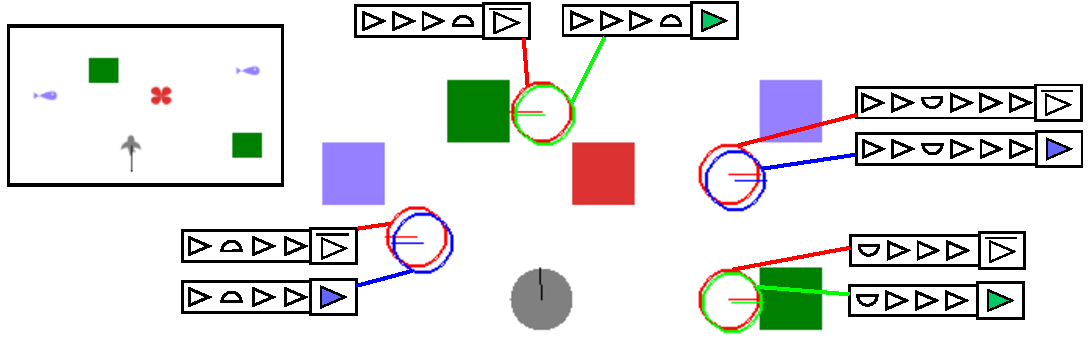
\includegraphics[scale=0.4]{img/detection.pdf}}
\caption{Distant affordances are detected and localized through sequences of interactions allowing to reach them. Circles show the position and orientation associated with these sequences (red: not moving forward, blue: eat, green: bump). 
We can notice that the agent ignores the alga since it has the same interactional property as an empty space.}
\label{fig:detect}
\end{figure}


\section{Conclusion and Future Work}\label{conclusion}

This work proposes a new mechanism to enable an interactionist agent to consider mobile and non-predictable entities in its emergent model of the environment. 
Results obtained in a simulated environment showed that the agent can still localize distant affordances without the notion of space, and define their positions in a similar way than in static environment, allowing the use of a Space Memory \cite{gay:space}.

Future work will study how the space memory can be used to better interact with other agents, and how the intrinsically motivated decisional mechanism can integrate probabilities of presence of affordance into consideration.
In multi-agent contexts, this will allow us to study the mutual integration of agents in each other's environmental model, and how these models can be exploited for generating behaviors involving collaborative tasks, such as coordinated hunt of large preys. 

We will also study how an agent can predict another agent's intentions through the observation of the other agent's context, as a previous implementation of the space memory demonstrated the possibility of reference change, opening intersubjectivity possibilities between agents.


\bibliographystyle{IEEEbib}
\bibliography{refs, refs_og}

\end{document}
